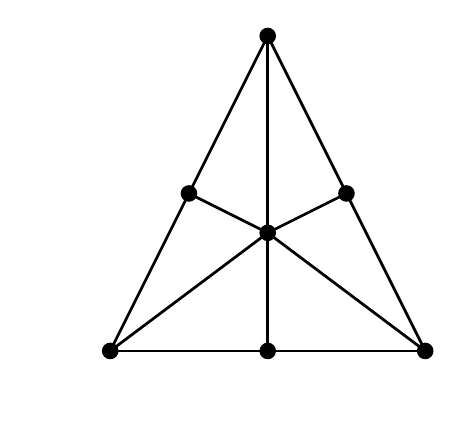
\begin{tikzpicture}[>=latex, scale=2, line width=1pt]
          % Coords
          \coordinate (V0) at (0,0);
          \coordinate (V1) at (2,0);
          \coordinate (V2) at (1,2);
          \coordinate (C01) at (1,0);
          \coordinate (C02) at (0.5,1);
          \coordinate (C12) at (1.5,1);
          \coordinate (C) at (1,0.75);
          % Arrows
          \draw[line width=1pt]
            (V0) -- (V1);
          \draw[line width=1pt]
            (V1) -- (V2);
          \draw[line width=1pt]
            (V2) -- (V0);
          \draw[line width=1pt]
            (V0) -- (C);
          \draw[line width=1pt]
            (V1) -- (C);
          \draw[line width=1pt]
            (V2) -- (C);
          \draw[line width=1pt]
            (C01) -- (C);
          \draw[line width=1pt]
            (C02) -- (C);
          \draw[line width=1pt]
            (C12) -- (C);
          % Points
          \fill (V0) circle (1.5pt);
          \fill (V1) circle (1.5pt);
          \fill (V2) circle (1.5pt);
          \fill (C01) circle (1.5pt);
          \fill (C02) circle (1.5pt);
          \fill (C12) circle (1.5pt);
          \fill (C) circle (1.5pt);


			%wegen abmessung
			          % Coords
          \coordinate (V0) at (0,0);
          \coordinate (V1) at (2,0);
          \coordinate (V2) at (1,2);
          \coordinate (C01) at (1,0);
          \coordinate (C02) at (0.5,1);
          \coordinate (C12) at (1.5,1);
          \coordinate (C) at (1,0.75);
          % Arrows
          \draw[opacity=0]
            (V0) -- (V1);
          \draw[opacity=0]
            (V1) -- (V2);
          \draw[opacity=0]
            (V2) -- (V0);
         
          % Points
          \fill[opacity=0](V0) node[below left] {\( \sigma^0 \)};
		  \fill[opacity=0](V0) node[above left] {\( c(\sigma^0) \)} circle (1.5pt);
          \fill[opacity=0, color=red] (V0)  circle (1.5pt);
          \fill[opacity=0] (V1)  circle (1.5pt);
          \fill[opacity=0](V2)   circle (1.5pt);
          \fill[opacity=0] (C02)  circle (1.5pt);
          \fill[opacity=0] (C01) node[below] {\( \sigma^1 \)};
		  \fill[opacity=0] (C01) node[above] {\( c(\sigma^1) \)} circle (1.5pt);
          \fill[opacity=0](C12)  circle (1.5pt);
          \fill[opacity=0](C) node[below] {\( \sigma^2\)};
		  \fill[opacity=0](C) node[above] {\( c(\sigma^2)\)} circle (1.5pt);	

		 \coordinate (CC2) at (1,1.25);
          \draw[opacity=0, ->] (CC2) + (135:0.15) arc (135:405:0.15) --++ (-3pt,3pt);
		
		\draw[opacity=0, ->] (V0) -- (V1);

		\coordinate (CC0) at (1,1.25);
          \draw[opacity=0, ->] (V0) + (135:0.1) arc (135:405:0.1) --++ (-2pt,2pt);

\end{tikzpicture}